\chapter{Evaluation}

\section{Results}

To determine how well the cSVD implementation performs, three tests benchmarks are made. The first test determines computational performance, the second test determines the Mean Squared Error (MSE) of the estimated singular values, and the third test determines the reconstruction error w.r.t. DNNs using ReLU activation functions.

To determine computational performance it is not necessary to use EDJMs (or other sparse matrices), the only computation time factor is the tensor size. The PyTorch cSVD is compared to the four cSVD implementations in Table \ref{tab:csvd:performance}, where the cSVD implementations are configured to estimate the 10\% largest singular values.

\begin{table}[H]
  \centering
    \begin{tabular}{|l|l|l|l|} \hline
      Implementation & Mean (s) & Variance & Mean speedup \\ \hline
      PyTorch SVD & 10.172 & 0.0082 & * \\ \hline
      Sequential cSVD & 1.0961  & 53.085e-03 & 9.280 \\ \hline
      Partially sequential cSVD & 1.095 & 97.853e-03 & 9.294 \\ \hline
      Batch cSVD & 0.034 & 2.872e-06 & 301.741 \\ \hline
      Batch cSVD (\texttt{gesvda}) & 0.037  & 0.149e-06 & 274.240 \\ \hline
    \end{tabular}
    \caption{Mean computation time, speedup and variance over   $25 \times 10000 \times 784$ tensor}
    \label{tab:csvd:performance}
\end{table}

To determine the MSE of the cSVD, it is necessary to determine how to calculate it for this case. The chosen method is shown in \eqref{eq:csvd:mse}. The range singular values below the 10\% threshold are not included in the calculation, which is why the largest $k$ singular values are used.

\begin{equation}
  \label{eq:csvd:mse}
    MSE = \frac{1}{k} \sum_{i=1}^{k} \left ( \frac{\hat \sigma_i - \sigma_i}{\sigma_i} \right )^2
\end{equation}

To compute the MSE, the four DNN configurations to create Table \ref{tab:dnn:score}. But because the accuracy of the DNNs are not important, because the only aspect required is the EDJMs are sparse. Therefore the DNNs are not trained until any specific accuracy, but just go through 20 epochs to ensure the EDJMs are sparse. Figure \ref{fig:csvd:mse} shows the MSE of the 40 EDJMs.
  
\begin{figure}[H]
  \centering
  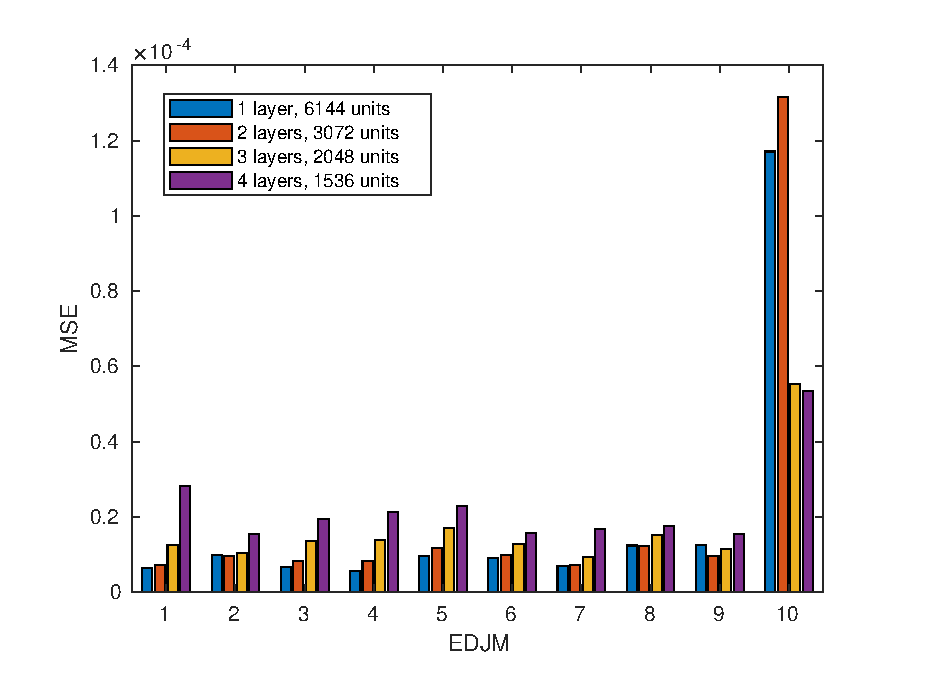
\includegraphics[scale=0.6]{Figures/csvd_mse.eps}
  \caption{cSVD MSE}
  \label{fig:csvd:mse}
\end{figure}

To compute the reconstruction error, Erichson, et. al., uses \eqref{eq:csvd:recon} \cite{erichson:csvd}. It can be regarded as the noise-to-signal ratio, as the numerator is the error and the denominator is a normalization using real signal.

\begin{equation}
  \label{eq:csvd:recon}
  ||X - USV^T||_F/||X||_F
\end{equation}



\begin{figure}[H]
  \centering
  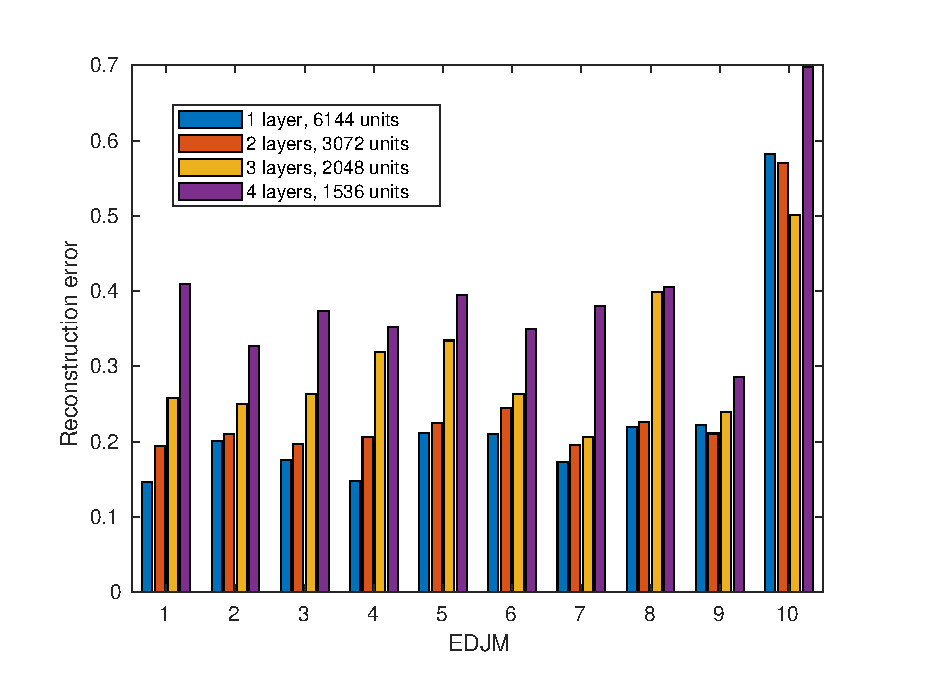
\includegraphics[scale=0.6]{Figures/csvd_reconstruction.eps}
  \caption{cSVD reconstruction}
  \label{fig:csvd:reconstruction}
\end{figure}

\begin{figure}[H]
  \centering
  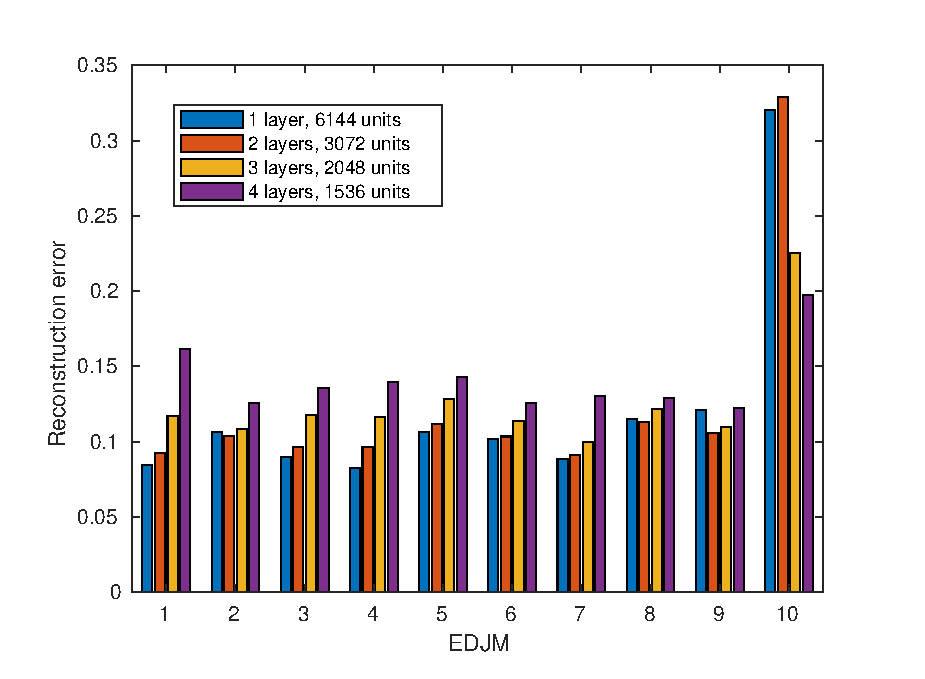
\includegraphics[scale=0.6]{Figures/svd_reconstruction.eps}
  \caption{SVD reconstruction}
  \label{fig:csvd:reconstruction}
\end{figure}

\section{Discussion}

\section{Conclusion}
